\documentclass[xcolor=pdftex,romanian,colorlinks]{beamer}

\usepackage[export]{adjustbox}
\usepackage{../tslides}
\usepackage[all]{xy}
\usepackage{pgfplots}
\usepackage{flowchart}
\usetikzlibrary{arrows,positioning,calc}
\lstset{language=Haskell}
\lstset{escapeinside={(*@}{@*)}}
\PrerenderUnicode{ăĂîÎȘșȚțâÂ}

\AtBeginSection[]{
  \begin{frame}
  \vfill
  \centering
  \begin{beamercolorbox}[sep=8pt,center,shadow=true,rounded=true]{title}
    \usebeamerfont{title}\insertsectionhead\par%
  \end{beamercolorbox}
  \vfill
  \end{frame}
}


\title[PF---Introducere]{Programare funcțională }
\subtitle{Introducere în programarea funcțională folosind Haskell}
\date{}
\begin{document}
\begin{frame}
  \titlepage
\end{frame}

\begin{frame}
\frametitle{}
\tableofcontents
\end{frame}

\begin{section}{Elemente de sintaxă}
\begin{frame}[fragile]{Sintaxă}
\begin{itemize}
\item Comentarii  
\small{\begin{asciihs}
-- comentariu pe o linie
{-  comentariu pe
    mai multe
    linii -}
\end{asciihs}}
\item Identificatori
\begin{itemize}
\item șiruri formate din litere, cifre, caracterele $\_$ și ' (apostrof)

\item identificatorii pentru variabile încep cu literă mică sau $\_$
\item identificatorii pentru tipuri și constructori încep cu literă mare
\item  Haskell este sensibil la majuscule (case sensitive)
\begin{asciihs}
double x =  2 * x
data Point a = Pt a a
\end{asciihs}
\end{itemize}
\end{itemize}

\end{frame}

\begin{frame}[fragile]{Sintaxă}
\begin{block}{Blocuri și indentare}
Blocurile sunt delimitate prin indentare.
\end{block}


\begin{asciihs}
fact n =  if n == 0
             then 1
             else  n * fact (n-1)

\end{asciihs}

\pause

\begin{asciihs}
trei =  let
             a = 1
             b = 2
        in a + b


\end{asciihs}
\pause
\begin{itemize}
\item echivalent, putem scrie
\begin{asciihs}
trei  =  let {a = 1; b = 2} in a + b
trei  =  let a = 1; b = 2 in a + b
\end{asciihs}
\end{itemize}
\end{frame}

\end{section}
%%%end Sintaxa

\begin{section}{Legarea variabilelor}
\begin{frame}[fragile]{Variabile}

 Presupunem că fisierul \verb"test.hs" conține
\begin{asciihs}
x=1
x=2
\end{asciihs}

\begin{itemize}
\item Ce valoare are  x?
\end{itemize}
\pause

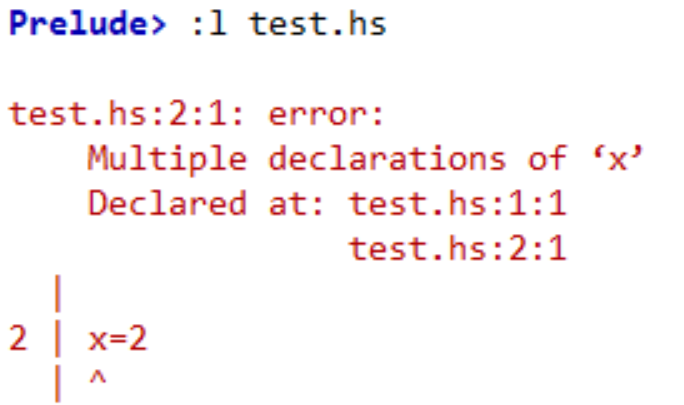
\includegraphics[scale=.9]{test.png}


\end{frame}

\begin{frame}[fragile]{Variabile}

\begin{block}{
În Haskell, variabilele sunt imuabile, adică:}
\end{block}

\begin{itemize}
\item \structure{=} $\,\,\,$ {\bf nu} este operator de atribuire
\medskip

\item \structure{{x = 1}} reprezintă o {\it legatură} (binding)
\medskip

\item din momentul în care o variabilă este legată la o valoare,

acea valoare nu mai poate fi schimbată


\end{itemize}


\end{frame}

\begin{frame}[fragile]{Legarea variabilelor}
\begin{block}{let .. in ...}
este o {\it expresie} care crează scop local
\end{block}
Presupunem că fișierul \verb"testlet.hs" conține
\begin{asciihs}
x=1
z= let x=3 in x
\end{asciihs}
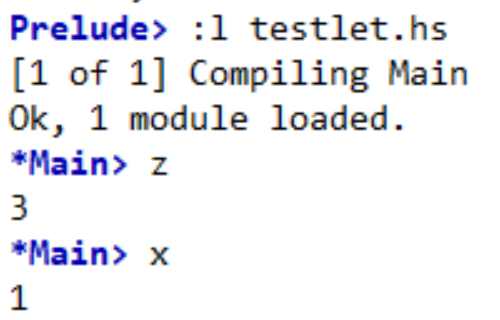
\includegraphics[height=3cm]{testlet.png}

\end{frame}

\begin{frame}[fragile]{Legarea variabilelor}
\begin{itemize}
\item {\bf let .. in ...}  crează scop local

\begin{minipage}{.4\columnwidth}
\begin{asciihs}
x = let
        z = 5
        g u = z + u
    in  let
            z = 7
        in g 0 + z
\end{asciihs}
\pause
\end{minipage}
\begin{minipage}{.4\columnwidth}
  \begin{asciihs}
   -- x=12
  \end{asciihs}
\end{minipage}
  \pause
\begin{minipage}{.8\columnwidth}
  \begin{asciihs}
x = let z = 5; g u = z + u in let z = 7 in g 0
\end{asciihs}
\end{minipage}
\pause
\begin{minipage}{.1\columnwidth}
  \begin{asciihs}
-- x=5
\end{asciihs}
\end{minipage}
\pause

\item clauza {\bf ... where ...} creaza scop local
\begin{asciihs}
f x = g x + g x + z
  where
    g x = 2*x
    z =  x-1

\end{asciihs}

\end{itemize}
\end{frame}

\begin{frame}[fragile]{Legarea variabilelor}
\begin{itemize}
\item {\bf let .. in ...}  este o expresie
\begin{asciihs}
x = [let y =8 in y, 9] -- x=[8,9]
\end{asciihs}

 \item {\bf where} este o clauză, disponibilă doar la nivel de definiție
 \begin{asciihs}
 (*@\color{red}x = [y where y =8, 9] -- error: parse error ...@*)
\end{asciihs}

\item Variabile pot fi legate și prin "pattern matching" la definirea unei funcții sau expresii {\bf case}.
\begin{columns}
\begin{column}{0.4\textwidth}
\begin{asciihs}
h x | x == 0   =  0
    | x == 1   = y + 1
    | x == 2   = y * y
    | otherwise = y
  where y = x*x
\end{asciihs}
\end{column}
\begin{column}{0.5\textwidth}
\begin{asciihs}
f x = case x of
             0 ->  0
             1 -> y + 1
             2 -> y * y
             _ -> y
  where y = x*x
\end{asciihs}
\end{column}
\end{columns}



\end{itemize}
\end{frame}

\end{section}
%%%end Legarea variabilelor


\begin{section}{Tipuri de date}

\begin{frame}[fragile]{Sistemul tipurilor}
\begin{block}{}
"There are three interesting aspects to types in Haskell:
 they are strong, they are static, and they can be automatically inferred."\\
\small{\url{http://book.realworldhaskell.org/read/types-and-functions.html}}
\end{block}
\begin{description}
\vitem[tare]  garanteaza absenta anumitor erori
\vitem[static] tipul fiecari valori este calculat la compilare
\vitem[dedus automat] compilatorul deduce automat tipul fiecarei expresii

\begin{asciihs}
Prelude> :t [('a',1,"abc")]
[('a',1,"abc")] :: Num b => [(Char, b, [Char])]
\end{asciihs}

\end{description}

\end{frame}

\begin{frame}[fragile]{Sistemul tipurilor}
\begin{block}{Tipurile de baza}
Int, Integer, Float, Double, Bool, Char, String
\end{block}

\pause
\begin{itemize}
\item tipuri compuse: tupluri si liste
\begin{asciihs}
Prelude> :t :t ('a', True)
('a', True) :: (Char, Bool)

Prelude> :t ["ana", "ion"]
["ana", "ion"] :: [[Char]]
\end{asciihs}
\pause
\item tipuri noi definite de utilizator
\begin{asciihs}
data RGB = Rosu | Verde | Albastru
data Point a = Pt a a    -- tip parametrizat
                         -- a este variabila de tip
\end{asciihs}
\end{itemize}
\end{frame}


%\begin{frame}[fragile]{Diagrama claselor}{
%\url{https://en.wikibooks.org/wiki/Haskell/Classes_and_types}}
%\begin{center}
%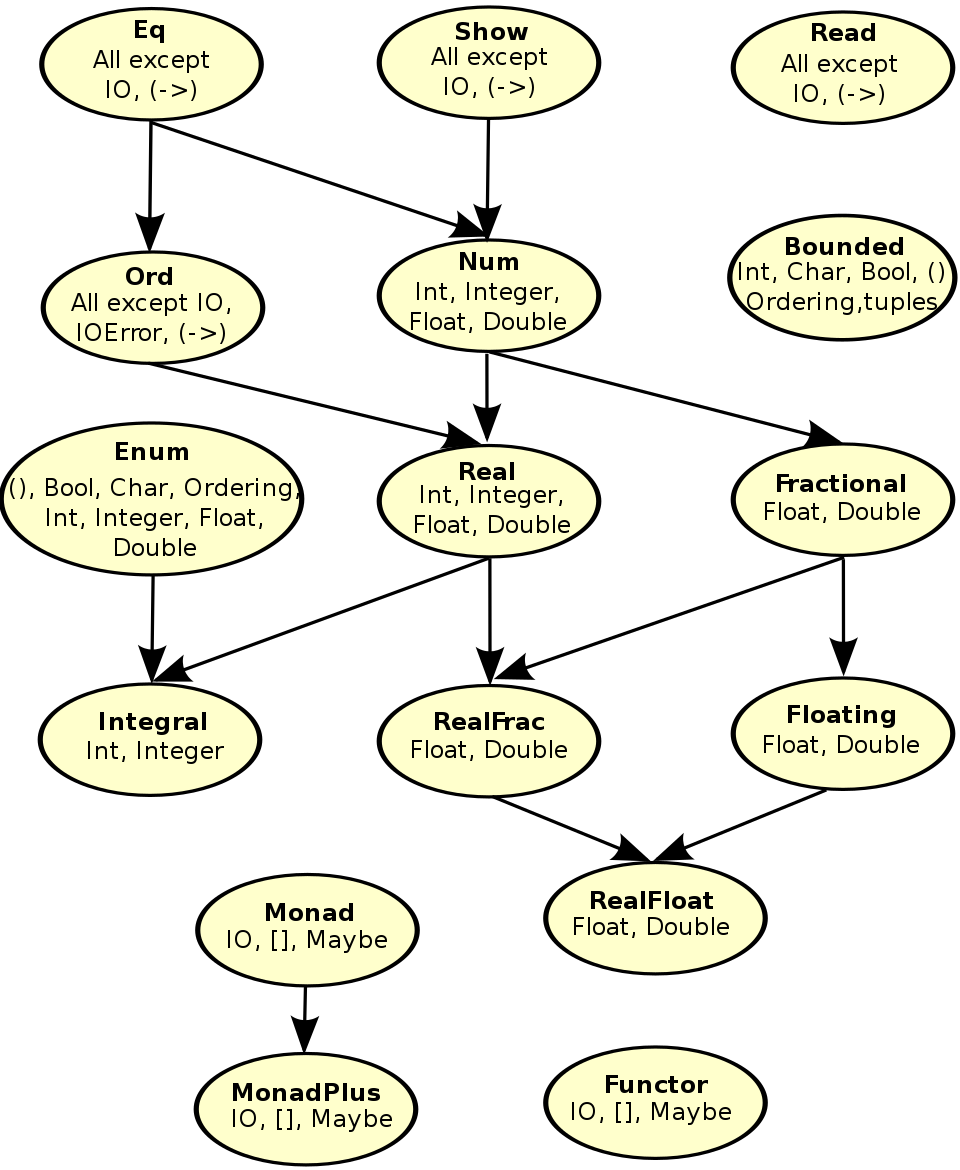
\includegraphics[height=6cm]{HC.png}
%\end{center}
%\end{frame}



\begin{frame}[fragile]{Tipuri de date}
\begin{itemize}
\item\structure{Integer}:  4, 0, -5
\begin{columns}
\begin{column}{0.4\textwidth}
\begin{asciihs}
Prelude> 4 + 3
Prelude> (+) 4 3
\end{asciihs}
\end{column}
\begin{column}{0.4\textwidth}
\begin{asciihs}
Prelude> mod 4 3
Prelude>  4 `mod` 3
\end{asciihs}
\end{column}
\end{columns}
\vitem\structure{Float}:  3.14
\begin{columns}
\begin{column}{0.4\textwidth}
\begin{asciihs}
Prelude> truncate 3.14
Prelude> sqrt 4
\end{asciihs}
\end{column}
\begin{column}{0.5\textwidth}
\begin{asciihs}
Prelude> let x = 4 :: Int
Prelude> sqrt (fromIntegral x)
\end{asciihs}
\end{column}
\end{columns}
\vitem\structure{Char}: 'a','A', '\textbackslash n'
%\begin{columns}
%\begin{column}{0.4\textwidth}
\begin{asciihs}
Prelude> import Data.Char
Prelude Data.Char> chr 65
Prelude Data.Char> ord 'A'
Prelude Data.Char> toUpper 'a'
Prelude Data.Char> digitToInt '4'
\end{asciihs}
%\end{column}
%\end{columns}
\end{itemize}
\end{frame}

\begin{frame}[fragile]{Tipuri de date}
\begin{itemize}
\item\structure{Bool}:  True, False
\begin{asciihs}
data Bool = True | False
\end{asciihs}
\begin{columns}
\begin{column}{0.5\textwidth}
\begin{asciihs}
Prelude> True && False || True
Prelude> not True

\end{asciihs}
\end{column}
\begin{column}{0.4\textwidth}
\begin{asciihs}
Prelude> 1 /= 2
Prelude> 1 == 2
\end{asciihs}
\end{column}
\end{columns}

\vitem\structure{String}:  "prog$\backslash$ndec"
\begin{asciihs}
type String = [Char] -- sinonim pentru tip
\end{asciihs}
\begin{columns}
\begin{column}{0.4\textwidth}
\begin{asciihs}
Prelude> "aa"++"bb"
"aabb"
Prelude> "aabb" !! 2
'b'
\end{asciihs}
\end{column}
\begin{column}{0.5\textwidth}
\begin{asciihs}
Prelude> lines "prog\ndec"
["prog","dec"]
Prelude> words "pr og\nde cl"
["pr","og","de","cl"]
\end{asciihs}
\end{column}
\end{columns}
\end{itemize}
\end{frame}

\begin{frame}{Liste}{Definiție}
\begin{block}{Listele sunt accesate de la stănga la dreapta}
Orice listă poate fi scrisă folosind doar constructorul \structure{(:)} și lista vidă \structure{[]}
\begin{itemize}
\item\ [1,2,3] == 1 : (2 : (3 : [])) == 1 : 2 : 3 : []
\item "abcd" == ['a','b','c','d'] == 'a' : ('b' : ('c' : ('d' : []))) == 'a' : 'b' : 'c' : 'd' : []
\end{itemize}
\end{block}
\vfill
\begin{block}{Definiție recursivă}
O \structure{listă} este
\begin{itemize}
\item \structure{vidă}, notată \structure{[]}; sau
\item \structure{compusă}, notată \structure{x:xs}, dintr-un un element \structure{x} numit \structure{capul listei (head)} și o listă \structure{xs} numită \structure{coada listei (tail)}.
\end{itemize}
\end{block}
\vfill
\end{frame}

\begin{frame}[fragile]{Tipuri de date compuse}
\begin{itemize}
\vitem Tipul \structure{listă}
\begin{asciihs}
Prelude>:t [True, False, True]
[True, False, True] :: [Bool]

\end{asciihs}

\item Tipul \structure{tuplu} - secvențe de de tipuri deja existente
\begin{asciihs}
Prelude> :t (1 :: Int, 'a', "ab")
(1 :: Int, 'a', "ab") :: (Int, Char, [Char])

Prelude> fst (1,'a') -- numai pentru perechi
Prelude> snd (1,'a')
\end{asciihs}

\vitem  Tipul \structure{unit}
\begin{asciihs}
Prelude> :t ()
() :: ()
\end{asciihs}

\end{itemize}
\end{frame}

\begin{frame}[fragile]{Tipuri. Clase de tipuri. Variabile de tip}

Ce răspuns primim in GHCi dacă introducem comanda
\begin{asciihs}
Prelude> :t 1
\end{asciihs}
\pause

Răspunsul primit este:
 \begin{asciihs}
 1 :: Num a => a
 \end{asciihs}

Semnificația este următoarea:

\begin{itemize}
\item \structure{a} este un {\it parametru de tip}
\item \structure{Num} este o clasă de tipuri
\item \structure{1} este o valoare de tipul \structure{a} din clasa
\structure{Num}
\end{itemize}
\begin{asciihs}
Prelude> :t 1
1 :: Num a => a

Prelude> :t [1,2,3]
[1,2,3] :: Num t => [t]

\end{asciihs}




\end{frame}



\end{section} %Tipuri

\begin{section}{Funcții}



\begin{frame}{Funcții în Haskell. Terminologie}
\begin{block}{Prototipul funcției \hfill
{\color{black}{\bf double} {:: Integer -> Integer}}}
\begin{itemize}
\item {\bf numele funcției}
\item signatura funcției
\end{itemize}
\end{block}
\begin{block}{Definiția funcției \hfill {\color{black}{\bf double}} \alert{elem} {\color{black}= elem + elem}}

\begin{itemize}
\item {\bf numele funcției}
\item \alert{parametrul formal}
\item corpul funcției
\end{itemize}
\end{block}
\begin{block}{Aplicarea funcției \hfill {\color{black}{\bf double}} \alert{5}}
\begin{itemize}
\item {\bf numele funcției}
\item \alert{parametrul actual (argumentul)}
\end{itemize}
\end{block}
\end{frame}

\begin{frame}{Exemplu: funcție cu două argumente}
\begin{block}{Prototipul funcției \hfill
{\color{black}{\bf add} {:: Integer -> Integer  -> Integer}}}
\begin{itemize}
\item {\bf numele funcției}
\item signatura funcției
\end{itemize}
\end{block}
\begin{block}{Definiția funcției \hfill {\color{black}{\bf add}} \alert{elem1} \alert{elem2} {\color{black}= elem1 + elem2}}

\begin{itemize}
\item {\bf numele funcției}
\item \alert{parametrii formali}
\item corpul funcției
\end{itemize}
\end{block}
\begin{block}{Aplicarea funcției \hfill {\color{black}{\bf add}} \alert{3} \alert{7}}
\begin{itemize}
\item {\bf numele funcției}
\item \alert{argumentele}
\end{itemize}
\end{block}
\end{frame}

\begin{frame}{Exemplu: funcție cu {\bf un} argument de tip tuplu}
\begin{block}{Prototipul funcției \hfill
{\color{black}{\bf dist} {:: (Integer, Integer)  -> Integer}}}
\begin{itemize}
\item {\bf numele funcției}
\item signatura funcției
\end{itemize}
\end{block}
\begin{block}{Definiția funcției \hfill {\color{black}{\bf dist}} \alert{(elem1, elem2)} {\color{black}= abs (elem1 - elem2)}}

\begin{itemize}
\item {\bf numele funcției}
\item \alert{parametrul  formal}
\item corpul funcției
\end{itemize}
\end{block}
\begin{block}{Aplicarea funcției \hfill {\color{black}{\bf dist}} \alert{(elem1, elem2)}}
\begin{itemize}
\item {\bf numele funcției}
\item \alert{argumentul}
\end{itemize}
\end{block}
\end{frame}

\begin{frame}[fragile]{Tipuri de funcții}
\begin{asciihs}

Prelude> :t abs
abs :: Num a => a -> a
Prelude> :t div
div :: Integral a => a -> a -> a

Prelude> :t (:)
(:) :: a -> [a] -> [a]
Prelude> :t (++)
(++) :: [a] -> [a] -> [a]


Prelude> :t zip
zip :: [a] -> [b] -> [(a, b)]
\end{asciihs}
\end{frame}

\begin{frame}[fragile]{Definirea funcțiilor}
\begin{block}{}
\vspace{-2ex}
\begin{asciihs}
fact :: Integer -> Integer
\end{asciihs}
\end{block}
\begin{itemize}
\item \structure{Definiție folosind {\bf if}}

\begin{asciihs}
fact n = if n == 0 then 1
         else n * fact(n-1)
\end{asciihs}
\pause

\item \structure{Definiție folosind ecuații}

\begin{asciihs}
fact 0 = 1
fact n = n * fact(n-1)
\end{asciihs}
 \pause

\item \structure{Definiție folosind cazuri}

\begin{asciihs}
fact n
  | n == 0    = 1
  | otherwise = n * fact(n-1)
\end{asciihs}
\end{itemize}
\end{frame}

\begin{frame}[fragile]{\Sh abloane (patterns)}
\begin{itemize}
\item
\begin{asciihs}
x:y = [1,2,3] -- x=1 si y =[2,3]
\end{asciihs}
Observați că { :} este constructorul pentru liste.\pause
\item
\begin{asciihs}
(u,v)=('a',[(1,'a'),(2,'b')]) -- u='a',
                              -- v=[(1,'a'),(2,'b')]
\end{asciihs}
Observați că (,,) este constructorul pentru tupluri.\pause
\item Definitii folosind șabloane
\begin{asciihs}
selectie :: Integer -> String -> String
\end{asciihs}
\vspace{-3ex}
\begin{columns}[t]
  \begin{column}{.45\columnwidth}
\begin{asciihs}
-- case...of
selectie x s =
    case (x,s) of
        (0,_) -> s
        (1, z:zs) -> zs
        (1, []) -> []
        _ -> (s ++ s)
\end{asciihs}
  \end{column}
  \begin{column}{.45\columnwidth}
\begin{asciihs}
-- stil ecuational
selectie 0 s = s
selectie 1 (_:s) = s
selectie 1 "" = ""
selectie _ s = s + s
\end{asciihs}
  \end{column}
\end{columns}

\end{itemize}
\end{frame}
\begin{frame}[fragile]{Tipuri de funcții}

Fie {foo} o funcție cu următorul tip


\begin{asciihs}
foo :: a -> b -> [a] -> [b]
\end{asciihs}


\begin{itemize}

\item are trei argumente, de tipuri a, b și [a]
\item întoarce un rezultat de tip [b]
\end{itemize}
\pause

Schimbăm signatura funcției astfel:

\begin{asciihs}
ffoo :: (a -> b) -> [a] -> [b]
\end{asciihs}



\begin{itemize}

\item are două argumente, de tipuri (a -> b) și [a],

adică o funcție de la a la b și o listă de elemente de tip a
\item întoarce un rezultat de tip [b]
\end{itemize}
\pause
\begin{asciihs}
Prelude> :t map
map :: (a -> b) -> [a] -> [b]

\end{asciihs}
\end{frame}



\end{section}

%-----------------------------------------------------
\begin{section}{Liste}
\begin{frame}{Liste}{Definiție}
\begin{block}
{Observație}
Orice listă poate fi scrisă folosind doar constructorul \structure{(:)} și lista vidă \structure{[]}
\begin{itemize}
\item\ [1,2,3] == 1 : (2 : (3 : [])) == 1 : 2 : 3 : []
\item "abcd" == ['a','b','c','d'] == 'a' : ('b' : ('c' : ('d' : []))) == 'a' : 'b' : 'c' : 'd' : []
\end{itemize}
\end{block}
\vfill
\begin{block}{Definiție recursivă}
O \structure{listă} este
\begin{itemize}
\item \structure{vidă}, notată \structure{[]}; sau
\item \structure{compusă}, notată \structure{x:xs}, dintr-un un element \structure{x} numit \structure{capul listei (head)} și o listă \structure{xs} numită \structure{coada listei (tail)}.
\end{itemize}
\end{block}
\vfill
\end{frame}

\begin{frame}[fragile]{Definirea listelor. Operații}
\begin{block}{ Intervale și progresii}
\begin{asciihs}
interval = ['c'..'e']       -- ['c','d','e']
progresie = [20,17..1]      -- [20,17,14,11,8,5,2]
progresie' = [2.0,2.5..4.0] -- [2.0,2.5,3.0,3.5,4.0]
\end{asciihs}
\end{block}
\pause
\begin{block}{Operații}
\begin{asciihs}
Prelude> [1,2,3] !! 2
3
Prelude> "abcd" !! 0
'a'
Prelude> [1,2] ++ [3]
[1,2,3]
Prelude> import Data.List
\end{asciihs}
\end{block}
\end{frame}

\begin{frame}[fragile]{Definiția prin selecție $\{x\mid P(x)\}$}
\structure{[E(x)| x <- [x1,…,xn], P(x)]}

\begin{asciihs}
Prelude> let xs = [0..10]
Prelude> [x | x <- xs, even x](*@\pause@*)
[0,2,4,6,8,10]

Prelude> let xs = [0..6]
Prelude> [(x,y) | x <- xs, y <- xs,  x + y == 10](*@\pause@*)
[(4,6),(5,5),(6,4)]
\end{asciihs}
Folosirea lui \structure{\tt{let}} pentru declarații locale:
\begin{asciihs}
Prelude> [(i,j) | i <- [1..2], (*@\color{blue}{let}@*) k = 2 * i, j <- [1..k]](*@\pause@*)
[(1,1),(1,2),(2,1),(2,2),(2,3),(2,4)]

Prelude> let xs = ['A'..'Z']
Prelude> [x | (i,x) <- [1..] `zip` xs, even i](*@\pause@*)
"BDFHJLNPRTVXZ"
\end{asciihs}

\end{frame}


\begin{frame}[fragile]{zip xs ys}
\begin{asciihs}
Prelude> let xs = ['A'..'Z']
Prelude> [x | (i,x) <- [1..] `zip` xs, even i](*@\pause@*)
"BDFHJLNPRTVXZ"

Prelude> :t zip
zip :: [a] -> [b] -> [(a, b)]

Prelude> let ys = ['A'..'E']
Prelude> zip [1..]  ys
[(1,'A'),(2,'B'),(3,'C'),(4,'D'),(5,'E')]
\end{asciihs}

\medskip\pause

\structure{Observați diferența!}

\begin{asciihs}
Prelude> zip [1..3] ['A'..'D']
[(1,'A'),(2,'B'),(3,'C')]

Prelude> [(x,y) | x <- [1..3], y <- ['A'..'D']]
[(1,'A'),(1,'B'),(1,'C'),(1,'D'),(2,'A'),(2,'B'),(2,'C'),(2,'D'),(3,'A'),(3,'B'),(3,'C'),(3,'D')]
\end{asciihs}

\end{frame}

\begin{frame}[fragile]{Lenevire (Lazyness)}

 Argumentele sunt evaluate doar când e necesar și doar cât e necesar


\begin{asciihs}
Prelude> head[]
*** Exception: Prelude.head: empty list
Prelude> let x = head []
Prelude> let f a = 5
Prelude> f x
5
Prelude> [1,head [],3] !! 0
1
Prelude> [head [],3] !! 1
*** Exception: Prelude.head: empty list
\end{asciihs}

\end{frame}

\begin{frame}[fragile]{Liste infinite}


\begin{block}{}

Drept consecință a \structure{evaluării leneșe}, se pot defini liste infinite (fluxuri de date)
\end{block}

\begin{asciihs}
Prelude> let natural = [0 ..]
Prelude> take 5 natural
[0,1,2,3,4]
\end{asciihs}
\pause
\begin{asciihs}
Prelude> let evenNat = [0, 2 ..] -- progresie infinita
Prelude> take 7 evenNat
[0,2,4,6,8,10,12]
\end{asciihs}
\pause
\begin{asciihs}
Prelude> let ones = [1,1..]
Prelude> let zeros = [0,0..]
Prelude> let both = zip ones zeros
Prelude> take 5 both
[(1,0),(1,0),(1,0),(1,0),(1,0)]
\end{asciihs}


\end{frame}





\end{section}










 \begin{frame}
  \vfill
  \centering
  \begin{beamercolorbox}[sep=8pt,center,shadow=true,rounded=true]{title}
    \usebeamerfont{title} Pe săptămâna viitoare! \par%
  \end{beamercolorbox}
  \vfill
  \end{frame}

\end{document}


%--- CE AM SCOS DIN CURSUL VECHI ------------

\begin{frame}[fragile]{Funcțiile sunt valori}{Funcțiile --- „cetățeni de rangul I”}
 Funcțiile sunt valori

 care pot fi trimise  ca argument sau întoarse ca rezultat

\begin{asciihs}
flip :: (a -> b -> c) -> (b -> a -> c)
\end{asciihs}
\begin{itemize}
\item definiția cu lambda expresii
\begin{asciihs}
flip f = \ x y -> f y x
\end{asciihs}
\item definiția folosind șabloane
\begin{asciihs}
flip f x y = f y x
\end{asciihs}
\item {\bf flip} ca valoare de tip funcție
\begin{asciihs}
flip = \ f x y -> f y x
\end{asciihs}

\end{itemize}

\end{frame}

\begin{frame}[fragile]{Tipuri. Clase de tipuri. Variabile de tip}

\begin{block}{O {\em clasă de tipuri} este o colecție de operații (o interfață).}

În clasa {\bf Num} regăsim acele date care au definite operațiile de adunare, scădere, înmulțire, etc.
\begin{asciihs}
  Prelude> :i Num
  class Num a where
    (+) :: a -> a -> a
    (-) :: a -> a -> a
    (*) :: a -> a -> a
    negate :: a -> a
    abs :: a -> a
    signum :: a -> a
    fromInteger :: Integer -> a
  instance Num Integer -- Defined in 'GHC.Num'
  instance Num Int -- Defined in 'GHC.Num'
  instance Num Float -- Defined in 'GHC.Float'
  instance Num Double -- Defined in 'GHC.Float'
\end{asciihs}
\end{block}

\end{frame}

\begin{frame}[fragile]{Funcții de ordin înalt}
{map, filter, foldl, foldr}
\begin{asciihs}
Prelude> map (*3) [1,3,4]
[3,9,12]
Prelude> filter (>=2) [1,3,4]
[3,4]
Prelude> foldr (*) 1  [1,3,4]
12
Prelude> foldl (flip (:)) [] [1,3,4]
[4,3,1]
\end{asciihs}

\begin{block}{Compunere si aplicare}
\begin{asciihs}
Prelude> map (*3) ( filter (<=3) [1,3,4])
[3,9]
Prelude> map (*3) . filter (<=3)  [1,3,4]
[3,9]
\end{asciihs}
\end{block}
\end{frame}



\begin{frame}[fragile]{Simplificăm definiția}
\begin{asciihs}
f :: [Int] -> Int
f xs = foldr (+) 0 (map sqr (filter pos xs))
  where
    sqr x = x * x
    pos x = x > 0
\end{asciihs}
\begin{alertblock}{Simplificare incorectă}
\begin{asciihs}
f :: [Int] -> Int
f xs = foldr (+) 0 (map (*@\color{red}{(x * x)} @*) (filter (*@\color{red}{(x > 0)}@*) xs))
\end{asciihs}
\end{alertblock}
\onslide<2>
\begin{block}{Simplificare corectă}
\begin{asciihs}
f :: [Int] -> Int
f xs = foldr (+) 0 (map (*@\color{blue}(\textbackslash\; x -> x * x) @*) (filter (*@\color{blue}{(\textbackslash\; x -> x > 0)} @*) xs))
\end{asciihs}
\end{block}
\end{frame}



\end{section}





